\documentclass[twocolumn,a4j]{jsarticle}
\setlength{\topmargin}{-20.4cm}
\setlength{\oddsidemargin}{-10.4mm}
\setlength{\evensidemargin}{-10.4mm}
\setlength{\textwidth}{18cm}
\setlength{\textheight}{26cm}

\usepackage[top=15truemm,bottom=25truemm,left=15truemm,right=15truemm]{geometry}
\usepackage[latin1]{inputenc}
\usepackage{amsmath}
\usepackage{amsfonts}
\usepackage{amssymb}
\usepackage[dvipdfmx]{graphicx}
\usepackage[dvipdfmx]{color}
\usepackage{listings}
\usepackage{listings,jvlisting}
\usepackage{geometry}
\usepackage{framed}
\usepackage{color}
\usepackage[dvipdfmx]{hyperref}
\usepackage{ascmac}
\usepackage{enumerate}
\usepackage{tabularx}
\usepackage{cancel}
\usepackage{scalefnt}

\renewcommand{\figurename}{Fig.}
\renewcommand{\tablename}{Table }

\lstset{
basicstyle={\ttfamily},
identifierstyle={\small},
commentstyle={\smallitshape},
keywordstyle={\small\bfseries},
ndkeywordstyle={\small},
stringstyle={\small\ttfamily},
frame={tb},
breaklines=true,
columns=[l]{fullflexible},
xrightmargin=0zw,
xleftmargin=3zw,
numberstyle={\scriptsize},
stepnumber=1,
numbersep=1zw,
lineskip=-0.5ex
}

\makeatletter
\def\@maketitle
{
\begin{center}
{\LARGE \@title \par}
\end{center}
\begin{flushright}
{\large 報告書 NO.07 - 1\quad\@date\quad\@author}
\end{flushright}
\par\vskip 1.5em
}
\makeatother

\setcounter{tocdepth}{3}

\author{来代 勝胤}
\title{令和3年度 11月 第1週 報告書}
\date{2021/11/4}

\begin{document}
\columnseprule=0.1mm

\maketitle
\section*{報告内容}
\begin{enumerate}[1.]
    \item 進捗状況
    \item ストレインアンプの調整
\end{enumerate}
\section{進捗状況}
今週は,ストレインアンプの調整を行った.
ロードセルに使用しているアンプは,
以前の実験と同様に動作していたため
ひずみセンサに取り付けられたアンプの調整を行った.
\section{ストレインアンプの調整}
以下のFig.1,Fig.2に2021年6月21日に行った
ロードセルとひずみセンサの校正実験の結果を示す.
\begin{figure}[htbp]
    \footnotesize
    \begin{center}
        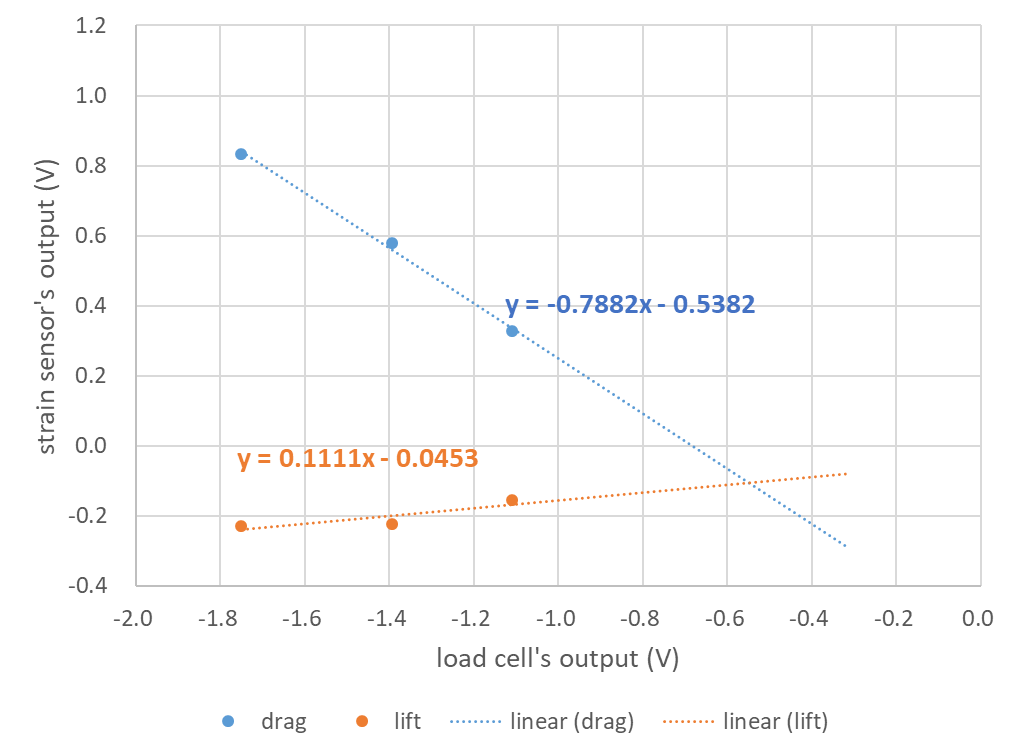
\includegraphics[width=80mm]{../images/previously_drag.png}
        \caption{previously data (drag)}
        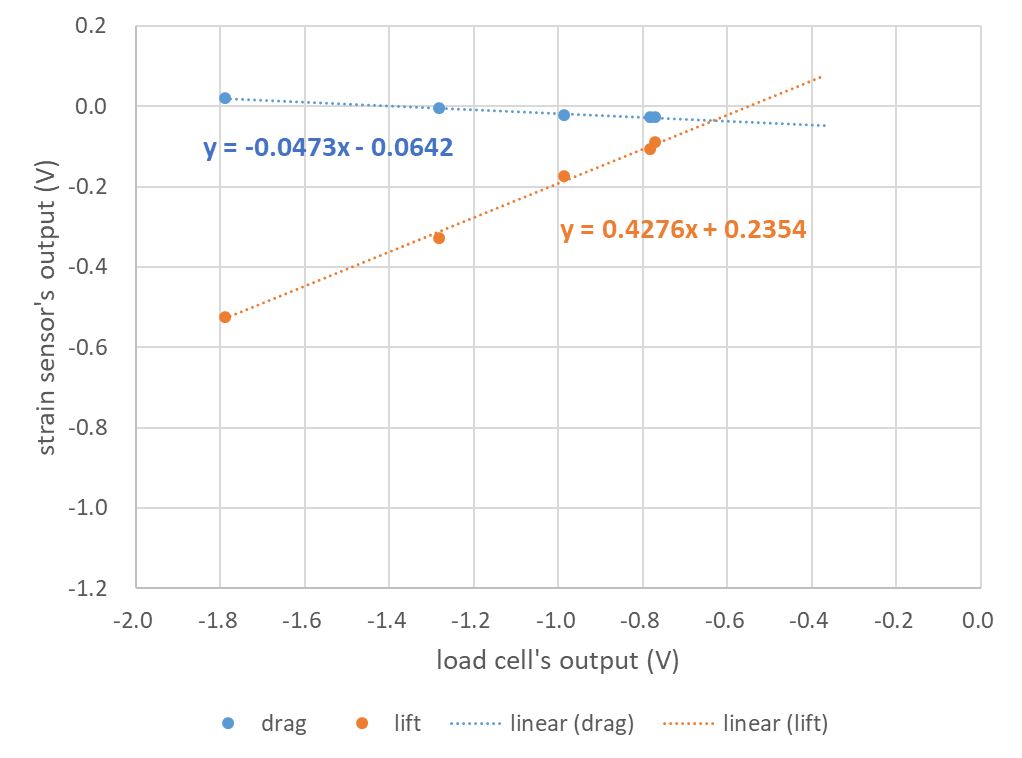
\includegraphics[width=80mm]{../images/previously_lift.png}
        \caption{previously data (lift)}
    \end{center}
\end{figure}\par
なお,今回の結果と比較するため,
ロードセルの出力電圧(横軸)は $0 ~ -2.0$ の範囲のデータを採用している.
\newpage
\subsection{Range:1k の場合}
以下のFig.3,Fig.4にレンジを「1k」として測定した結果を示す.
\begin{figure}[htbp]
    \footnotesize
    \begin{center}
        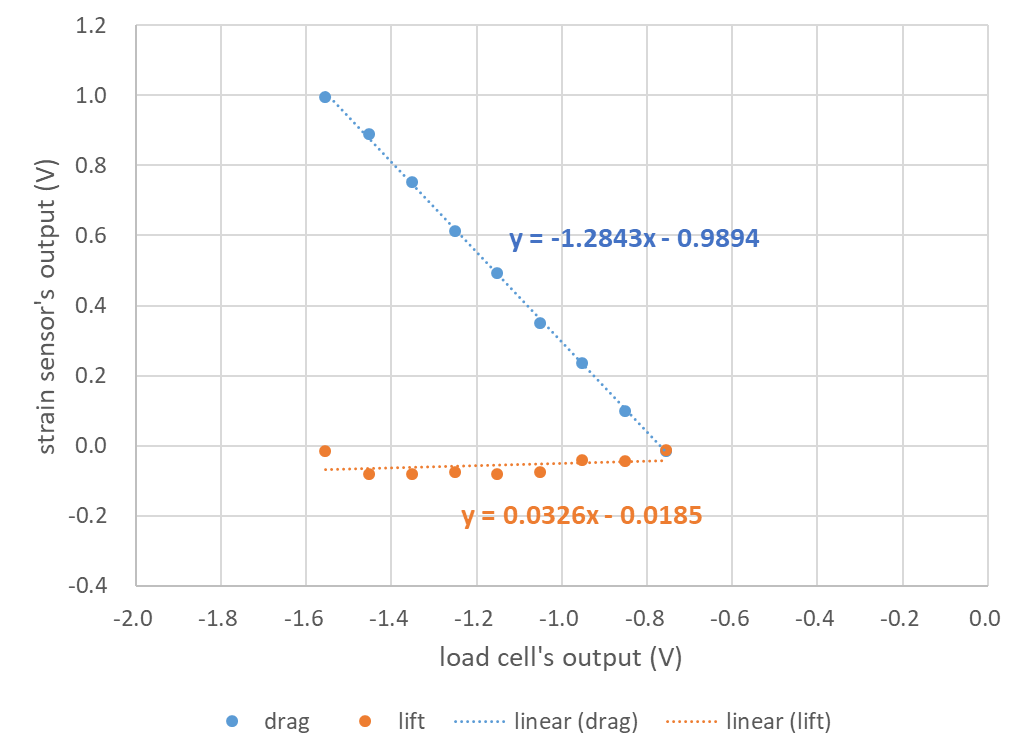
\includegraphics[width=80mm]{../images/1k_drag.png}
        \caption{range : 1k (drag)}
        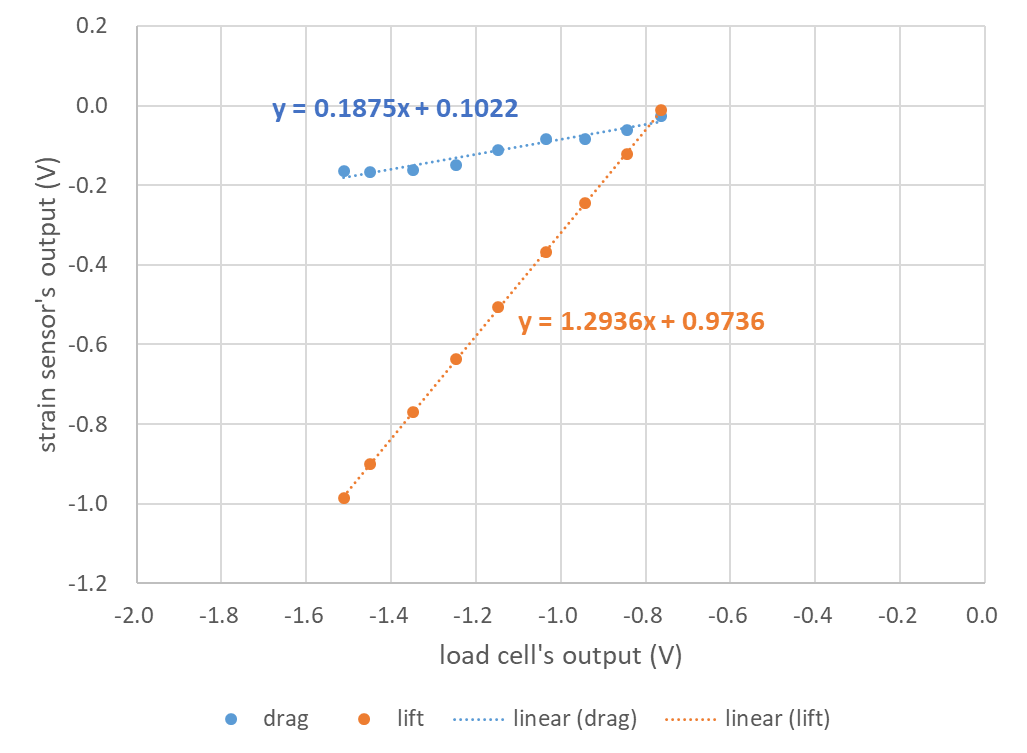
\includegraphics[width=80mm]{../images/1k_lift.png}
        \caption{range : 1k data (lift)}
    \end{center}
\end{figure}\par
Fig.3をみると,Fig.1と比較して,
近似式の傾きの差異は大きいが,
ひずみセンサの出力電圧(縦軸)の範囲と
同様の結果が得られていると考えられる.
供試体を押す角度によって,
結果が変化することを考慮してデータの解析を行う必要がある.
\newpage
\subsection{Range:2k の場合}
以下のFig.5,Fig.6にレンジを「2k」として測定した結果を示す.
\begin{figure}[htbp]
    \footnotesize
    \begin{center}
        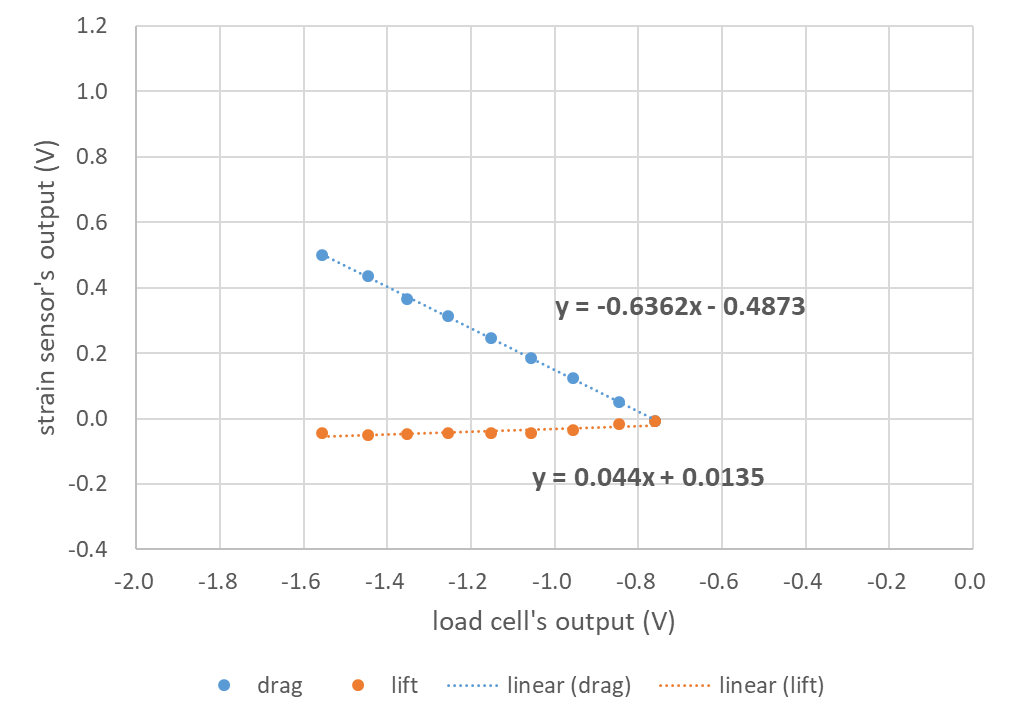
\includegraphics[width=80mm]{../images/2k_drag.png}
        \caption{range : 2k (drag)}
        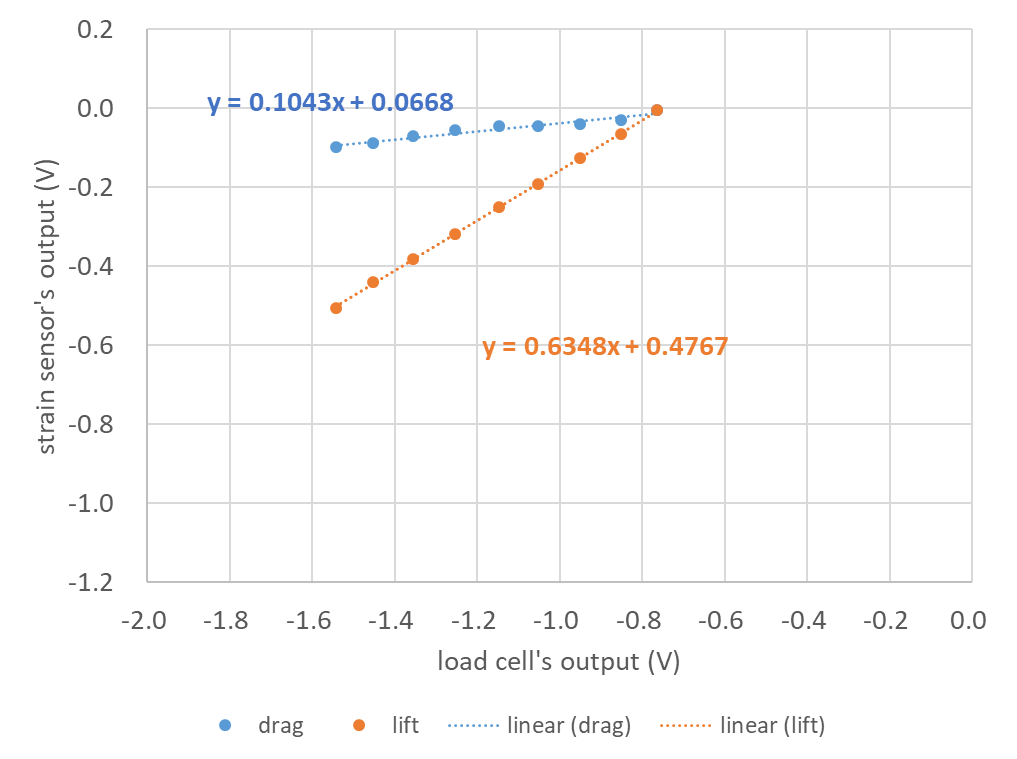
\includegraphics[width=80mm]{../images/2k_lift.png}
        \caption{range : 2k (lift)}
    \end{center}
\end{figure}\par
Fig.6をみると,Fig.2と比較して,ひずみセンサの出力電圧(縦軸)の範囲と
同様の結果が得られていると考えられる.
こちらもFig.1とFig.3の関係と同様に,
押す角度によって結果が大きく変化することを考慮する必要がある.
\newpage
\subsection{Range:500 の場合}
以下のFig.5,Fig.6にレンジを「500」として測定した結果を示す.
\begin{figure}[htbp]
    \footnotesize
    \begin{center}
        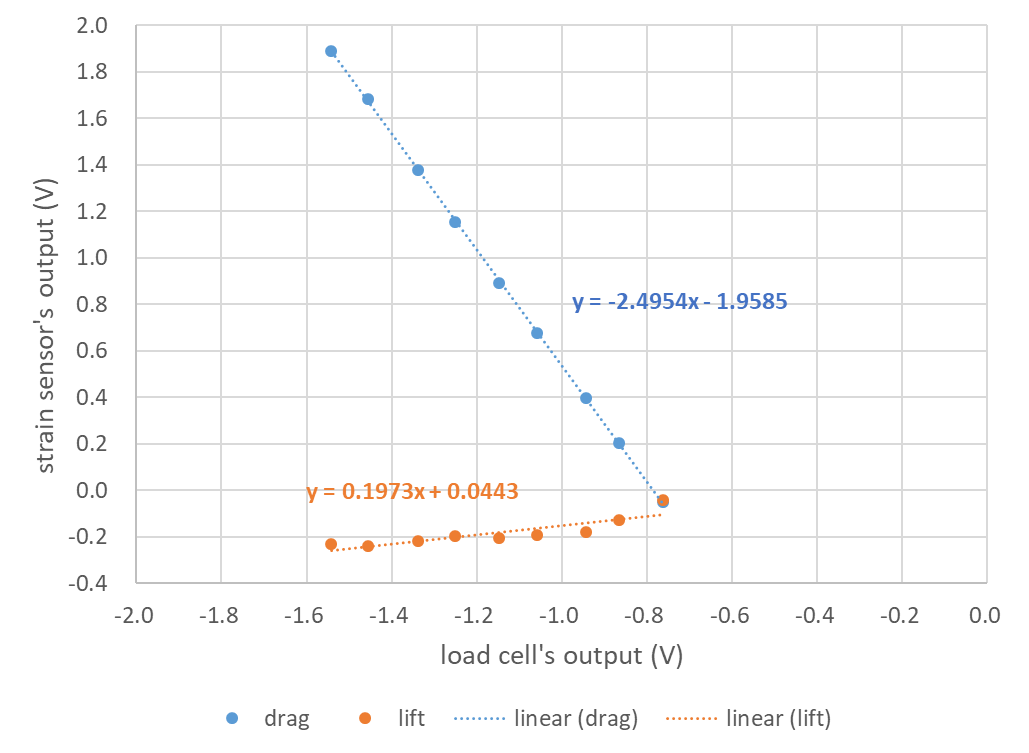
\includegraphics[width=80mm]{../images/500_drag.png}
        \caption{range : 500 (drag)}
        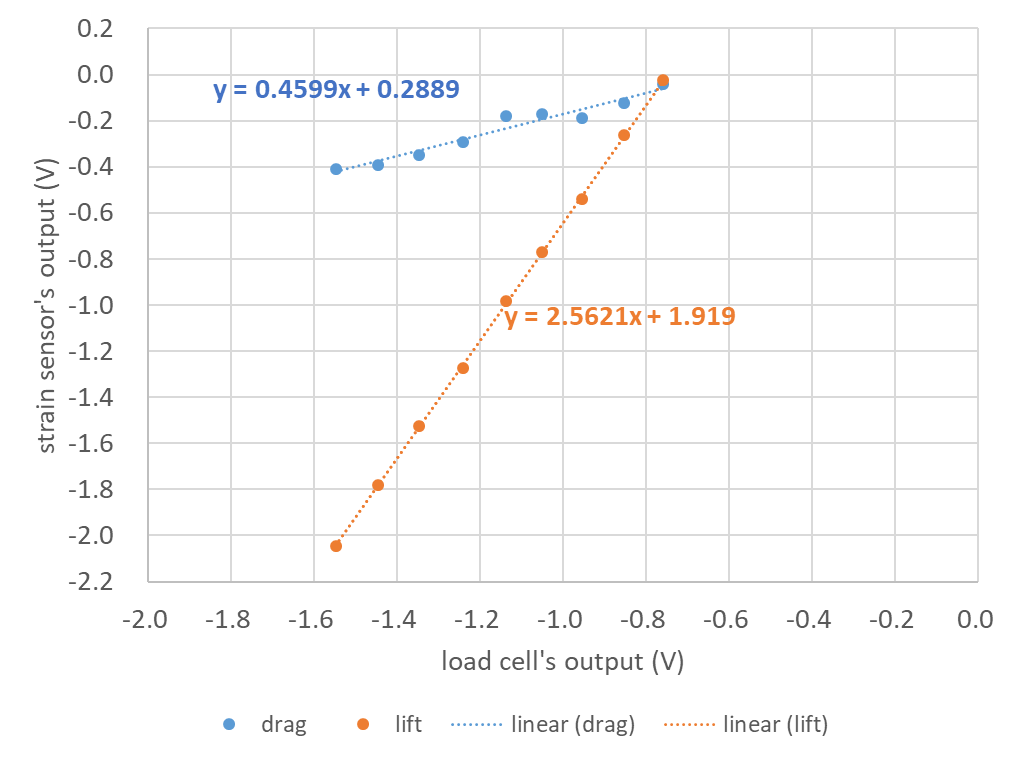
\includegraphics[width=80mm]{../images/500_lift.png}
        \caption{range : 500 (lift)}
    \end{center}
\end{figure}\par
ひずみセンサの出力電圧(縦軸)の範囲が,他のデータと大きく異なるため
以前の校正実験の際の設定に該当しないと考えられる.
\newpage
\subsection{合力の比較}
これまでの実験結果をみると,
力を加える方向の微細な差で,大きく結果が変化していることが考えられる.
そこで,抗力及び揚力方向のひずみセンサが90度に取り付けられていると仮定し,
以下の関係性から合力を算出した.
\begin{eqnarray*}
    F &=& \sqrt{f_x ^2 + f_y ^2} \\
    F &:& 合力\\
    f_x &:& 抗力\\
    f_y &:& 揚力\\
\end{eqnarray*}\par
Fig.1~Fig.8の測定結果から算出した合力を以下のFig.9,Fig.10に示す.
\begin{figure}[htbp]
    \footnotesize
    \begin{center}
        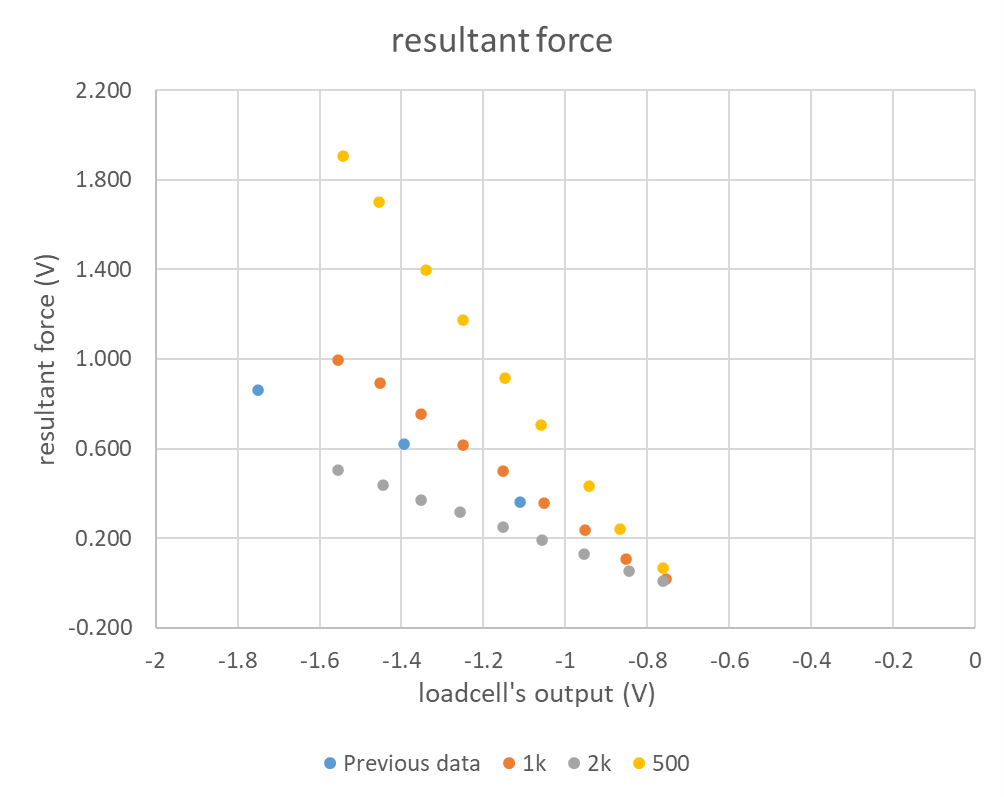
\includegraphics[width=80mm]{../images/resultantforce_drag.png}
        \caption{resultant force (drag)}
        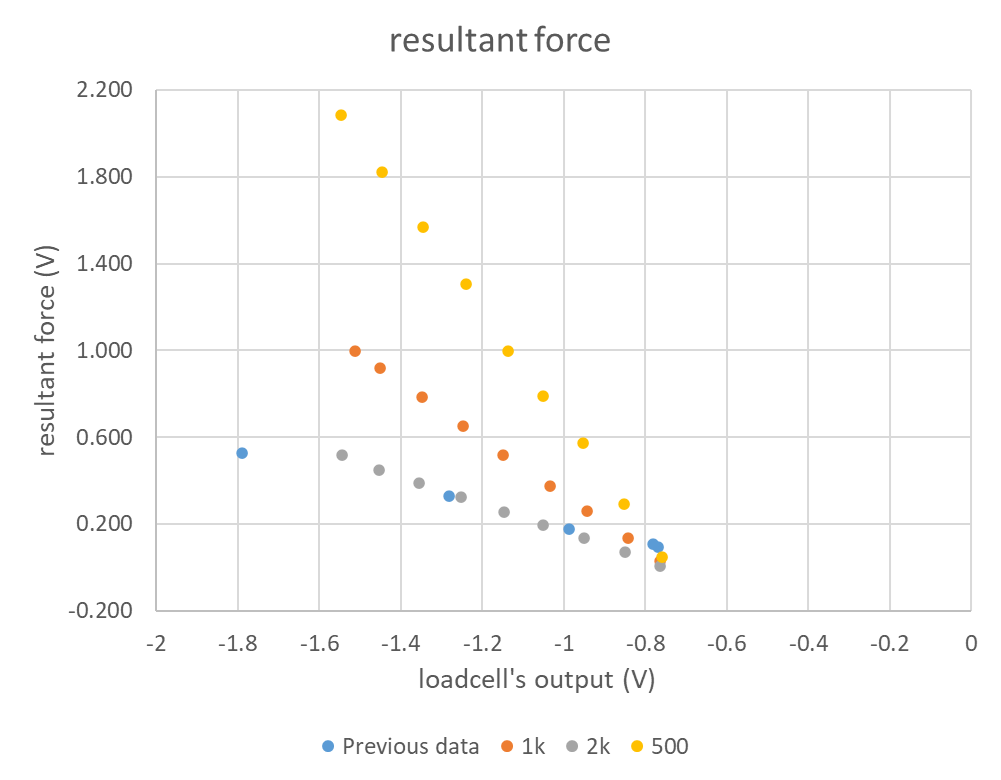
\includegraphics[width=80mm]{../images/resultantforce_lift.png}
        \caption{resultant force (lift)}
    \end{center}
\end{figure}\par
\end{document}